\documentclass[a4paper,10pt]{article}
\usepackage{graphicx}
\usepackage[left=1in,right=1in,top=1in,bottom=1in]{geometry}
\usepackage{hyperref}
\usepackage{fancyhdr}

\pagestyle{fancy}
\lhead{\textbf{Daniel Velarde Kubber}}
\rhead{\textbf{Curriculum Vitae}}
\cfoot{\thepage}

\begin{document}

% Add your photo in the upper right corner
\begin{minipage}[t]{0.7\textwidth}
  % Your existing content goes here
\end{minipage}
\hfill
\begin{minipage}[t]{0.3\textwidth}
  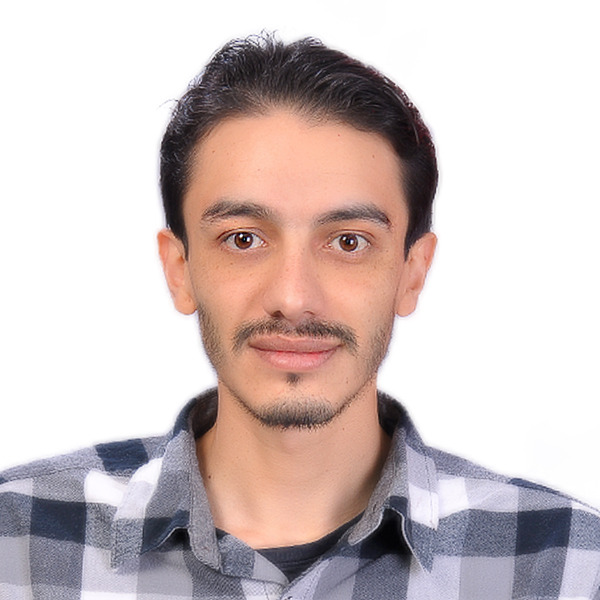
\includegraphics[width=2.5cm]{photocv.jpeg}
\end{minipage}

\begin{center}
\textbf{\LARGE Daniel Velarde Kubber}
\end{center}

\section*{Professional Summary}
Passionate about data and technology, I am a results-oriented professional with a background in Industrial and Systems Engineering. From my early days as a database administrator to my role as an entrepreneur and CEO at Hobbie 3D Print, I have honed my skills in data management, strategic leadership, and technical competence.

My professional journey, which includes hands-on experience in 3D printer programming, database administration, and project management, reflects my dedication to harnessing data to drive business success. I am driven by the power of innovation and thrive on the challenge of fostering growth.

With a strong commitment to data-driven decision-making, I am excited to apply my expertise to new opportunities and contribute to the fields of data engineering, data analysis, and data science.

\section*{Education}
\begin{tabular}{p{3cm}p{12cm}}
    2012 & Bachelor of Industrial and Systems Engineering, Universidad Privada Boliviana, Cochabamba, Bolivia \\
\end{tabular}

\section*{Licenses and Certifications}
\begin{description}
    \item[Certificate:] Introduction to Data Engineering, Coursera, August 2023
    \item[Certificate URL:] \url{https://www.coursera.org/account/accomplishments/certificate/9S9DAUQLBP27}
\end{description}

\vspace{1pt} % Adjust the value to control the amount of space

\begin{description}
    \item[Certificate:] Introduction to Relational Databases (RDBMS), Coursera, August 2023
    \item[Certificate URL:] \url{https://www.coursera.org/account/accomplishments/certificate/SG8MV2SLJXHC}
\end{description}

\vspace{1pt} % Adjust the value to control the amount of space

\begin{description}
    \item[Certificate:] Python for Data Science, Artificial Intelligence, and Development, Coursera, August 2023
    \item[Certificate URL:] \url{https://www.coursera.org/account/accomplishments/certificate/X6P3RHPT255M}
\end{description}

\vspace{1pt} % Adjust the value to control the amount of space

\begin{description}
    \item[Certificate:] Python Project for Data Engineering, Coursera, August 2023
    \url{https://www.coursera.org/account/accomplishments/certificate/WEQ4BMAGTZZN}
\end{description}

\vspace{1pt} % Adjust the value to control the amount of space

\begin{description}
    \item[Certificate:] Practical Introduction to Linux Commands and Shell Scripting, Coursera, September 2023
    \item[Certificate URL:] \url{https://www.coursera.org/account/accomplishments/certificate/TN4F6WG8DWKB}
\end{description}

\vspace{1pt} % Adjust the value to control the amount of space

\begin{description}
    \item[Certificate:] Databases and SQL for Data Science with Python, Coursera, September 2023
    \item[Certificate URL:] \url{https://www.coursera.org/account/accomplishments/certificate/AZMNGATPHMYT}
\end{description}

\vspace{1pt} % Adjust the value to control the amount of space

\begin{description}
    \item[Certificate:] Relational Database Administration (DBA), Coursera, September 2023
    \item[Certificate URL:] \url{https://www.coursera.org/account/accomplishments/certificate/EASM4DYAZY4L}
\end{description}

\vspace{1pt} % Adjust the value to control the amount of space

\begin{description}
    \item[Certificate:] ETL and Data Pipeline with Shell, Airflow, and Kafka, Coursera, September 2023
    \item[Certificate URL:] \url{https://www.coursera.org/account/accomplishments/certificate/HGASHU2DN99L}
\end{description}

\section*{Skills}
\begin{tabular}{p{4.5cm}p{4.5cm}p{4.5cm}}
    Databases & Data Architecture & Electronic Funds Transfer \\
    Database Security & Database Design & Import/Export Operations \\
    Database Administration & RDBMS & Inventory Management \\
    Database Servers & Data Pipeline & Inventory Control \\
    SQL & Data Visualization & Basic Accounting \\
    IBM Db2 & Bokeh & Project Management \\
    MySQL & Matplotlib & Digital Marketing \\
    NoSQL & Pandas & Microsoft Office \\
    ETL (Extract, Load, Transform) & NumPy & 3D Modeling \\
    Jupyter Notebook & IBM Cloud & 3D Printing \\
    Python & Linux & Product Development \\
    C++ & C\# & \\
    PostgreSQL & & \\
\end{tabular}

\section*{Interests}
In my free time, I have a passion for reading fantasy books, immersing myself in epic worlds reminiscent of "The Lord of the Rings" and "World of Warcraft." I also enjoy video games, both as a form of entertainment and as a way to connect with my children.

I am an avid learner and find joy in programming, exploring various programming languages, and, at one point, delving into game development with Unity. Additionally, I have a creative side that I express through painting miniatures
\end{document}